\section{Discussion}

\begin{frame}{Discussion}

    \begin{figure}
        \centering
        \begin{minipage}{.25\textwidth}
          \centering
          
\includegraphics[width=0.8\textwidth]{../../images/privacy.png}
        \end{minipage}%
        \begin{minipage}{.7\textwidth}
            Storing sensitive student data, as in the previous case, requires careful consideration 
            of data security and privacy (in human rights sense). 
            Some possible issues:
        \end{minipage}
    \end{figure}

    \begin{itemize}[<alert@+>]\color{gray}
        \item Compliance with Regulations: Ensure compliance with data protection regulations, such as GDPR, LGPD (Brazil), or other relevant laws
        \item Access Control
        \item User Consent, Transparency
        \item Secure Coding Practices
    \end{itemize}
    
\end{frame}

\begin{frame}{Our proposal}
    The traditional approach used to build dashboards (we are currently confirming through a Systematic Literature Review):

    \begin{table}[]
        \begin{tabular}{|l|l|l|} \hline
                 & Can choose Features? & Can see Predictions?\\ \hline
         Student & No                   & No                  \\ \hline
         Teacher & No                   & Yes                 \\ \hline
         Manager & Yes                  & Yes                 \\ \hline
        \end{tabular}
    \end{table}

    \pause
    Our proposal: Student \underline{in Control} Perspective
    \pause
    \begin{table}[]
        \begin{tabular}{|l|l|l|} \hline
                 & Can choose Features?  & Can see Predictions?                    \\ \hline
         Student & \textcolor{red}{Yes}  & \textcolor{red}{Yes}                    \\ \hline
         Teacher & No                    & \textcolor{blue}{Maybe} (student decides) \\ \hline
         Manager & No                    & \textcolor{blue}{Maybe} (student decides) \\ \hline
        \end{tabular}
    \end{table}

\end{frame}

\begin{frame}{Software Engineering}

    \begin{figure}
        \centering
        \begin{minipage}{.7\textwidth}
            Some issues this approach brings to software engineering:
        \end{minipage}%
        \begin{minipage}{.25\textwidth}
          \centering
          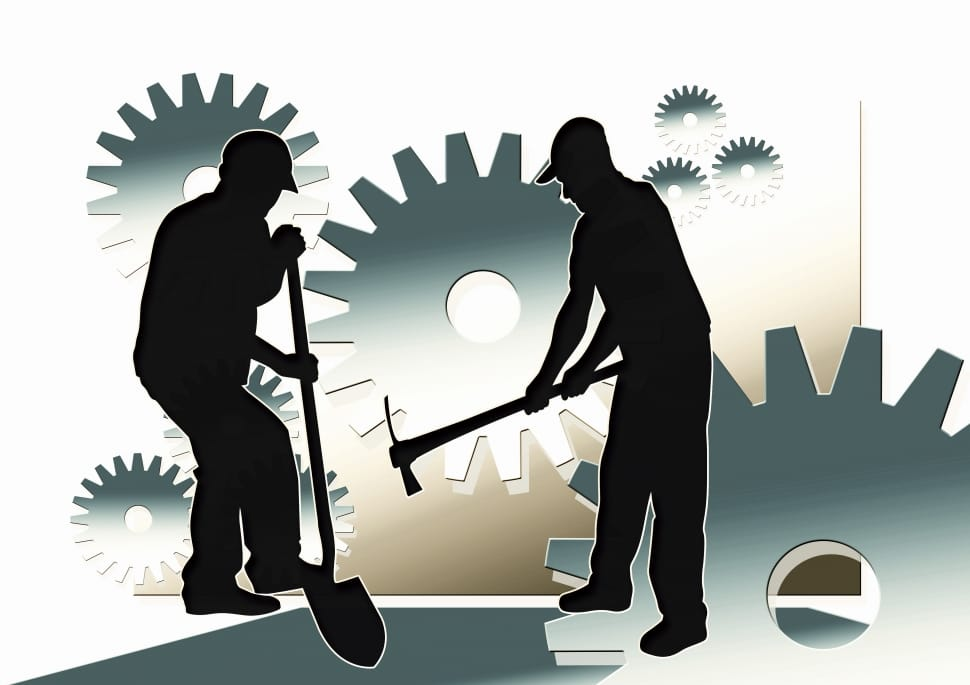
\includegraphics[width=0.8\textwidth]{../../images/work-workers-men.jpg}
        \end{minipage}
    \end{figure}

    \begin{itemize}[<+-|alert@+>]\color{gray}
        \item The Moodle Analytics API is designed primarily for teachers and managers, so a lot of 
              work is needed on plugins to empower students with similar capabilities
        \item The possibility for each student to choose their own indicators requires 
              rebuilding the model many times, which can impact performance
    \end{itemize}
\end{frame}

